%%% Test a table
%
% Set the \input{} to the table you want to test, then typeset this file
%
\documentclass[a4paper]{book}
%\documentclass[draft,a4paper]{book}
%% use [showframe] to show the frames
\usepackage[showframe]{geometry}
\usepackage{longtable}% Allow for split of the table over more than one page
\usepackage{rotating} % Make it possible to rotate headers
\usepackage[normal]{caption} % Keep captions to (long)tables normal sized
% must go *after* rotating package
\usepackage{booktabs} % To get nice table layout
%
% To include graphics in tables
\usepackage{graphicx}
%
%% Settings from the main text we also need for the test
\usepackage{fontspec}
\setmainfont{Hoefler Text}[]
%\setmainfont{Times New Roman}[]
\newfontfamily\greekfont{Times New Roman}
\newfontfamily\hebrewfont{Arial Hebrew}
\newfontfamily\arabicfont{Arial Unicode MS}
\usepackage[quiet]{polyglossia}
\setmainlanguage{latin}
\setotherlanguage{greek}
\setotherlanguage{hebrew}
\setotherlanguage{arabic}
%%% Special command for roman numerals
%% Usage: \rnum{<roman numeral>}
%% Example: \rnum{mdclxviii}
\newcommand{\rnum}[1]{%
\textsc{#1}%
}
%
\begin{document}
Lorem ipsum dolor sit amet, consectetur adipiscing elit, sed do eiusmod tempor
incididunt ut labore et dolore magna aliqua.
Ut enim ad minim veniam, quis nostrud exercitation ullamco laboris nisi ut
aliquip ex ea commodo consequat.
Duis aute irure dolor in reprehenderit in voluptate velit esse cillum dolore
eu fugiat nulla pariatur.
Excepteur sint occaecat cupidatat non proident, sunt in culpa qui officia
deserunt mollit anim id est laborum.

\begin{table}[htbp]
%\tiny
%\scriptsize
%\footnotesize
%\small
%\normalsize
\centering
%\setlength{\tabcolsep}{3pt}
%\renewcommand{\arraystretch}{1.3}
%%
%%%% Liber I p43
%%
%%% Count out columns for fixed-width source font
% 000000011111111112222222222333333333344444444445555555555666666666677777777778
% 345678901234567890123456789012345678901234567890123456789012345678901234567890
%
\begingroup
%% Select a general font size (uncomment one from the list)
%\tiny
\scriptsize
%\footnotesize
%\small
%\normalsize
%% Center the whole table left-right
\centering
%% Modify separation between columns
\setlength{\tabcolsep}{1.6pt}
%% Modify distance between rows
\renewcommand{\arraystretch}{1.2}
%
%% Define reference symbols
\newcommand{\da}{{\tiny †}}
\newcommand{\db}{{\tiny ‡}}
%% The angle with which to slant
\newcommand{\ang}{60}
%% Generate the column headers
\newcommand{\hdrs}{%
% A \multicolumn{} here would clash with \addcontentsline{}
\begin{rotate}{\ang}Anni periodi\end{rotate} &
&
\multicolumn{1}{c}{\begin{rotate}{\ang}\textgreek{Εκατομβαιών}\end{rotate}} & &
\multicolumn{1}{c}{\begin{rotate}{\ang}\textgreek{Μεταγειτνιών}\end{rotate}} & &
\multicolumn{1}{c}{\begin{rotate}{\ang}\textgreek{Βοηδρομιών}\end{rotate}} & &

\multicolumn{1}{c}{\begin{rotate}{\ang}\textgreek{Πυανεψιών}\end{rotate}} & &
\multicolumn{1}{c}{\begin{rotate}{\ang}\textgreek{Μαιμακτηριών}\end{rotate}} & &
\multicolumn{1}{c}{%
\begin{rotate}{\ang}\textgreek{Ποσειδεών \gnums{1}{α}}\end{rotate}} & &

\multicolumn{1}{c}{%
\begin{rotate}{\ang}\textgreek{Ποσειδεών \gnums{1}{β}}\end{rotate}} & &

\multicolumn{1}{c}{\begin{rotate}{\ang}\textgreek{Γαμηλιών}\end{rotate}} & &
\multicolumn{1}{c}{\begin{rotate}{\ang}\textgreek{Ανθεστηριών}\end{rotate}} & &
\multicolumn{1}{c}{\begin{rotate}{\ang}\textgreek{Ελαφηβολιών}\end{rotate}} & &

\multicolumn{1}{c}{\begin{rotate}{\ang}\textgreek{Μουνυχιών}\end{rotate}} & &
\multicolumn{1}{c}{\begin{rotate}{\ang}\textgreek{Θαργηλιών}\end{rotate}} & &
\multicolumn{1}{c}{\begin{rotate}{\ang}\textgreek{Σκιῤῥοφοριών}\end{rotate}} & &

\multicolumn{2}{l}{\begin{turn}{\ang}\textgreek{περιτταὶ ἡμέραι}\end{turn}} \\
}
%
%% Let longtable process the whole table in one go
\setcounter{LTchunksize}{100}
\begin{longtable}[c]{@{} r  r  *{13}{r@{~}l} r c @{}}
\toprule
\multicolumn{30}{c}{\Large\textsc{Tabula neomeniarum Atticarum}} \\
\multicolumn{30}{c}{\Large\textsc{in mensibus Iulianis}} \\
\toprule
% Put a reference to the first page of the table in the List of Tables
\addcontentsline{lot}{section}{%
\protect\numberline{\thetable}Neomeniarum Atticarum in mensibus Iulianis}
\label{tab:p043}
\hdrs % Column headers from the above definition
\midrule
\endfirsthead
%%
\toprule
\multicolumn{30}{c}{\Large\textsc{Residuum tabulae neomeniarum Atticarum}} \\
\multicolumn{30}{c}{\Large\textsc{in mensibus Iulianis}} \\
\toprule
\hdrs % Column headers from the above definition
\midrule
\endhead
%%
% The \nopagebreak commands result in a cline{} at the bottom of each page
% Putting in a bottomrule looks weird.
%\bottomrule
\addlinespace[5pt]
  & & & \multicolumn{11}{l}{\super\da \textgreek{ἐξαιρεσίμαίων [?]}}
& & & & \multicolumn{11}{l}{\super\db \textgreek{δισέξαιρεσιμαίων [?]}}
\\
\endfoot
%%
%\bottomrule
\addlinespace[5pt]
  & & & \multicolumn{11}{l}{\super\da \textgreek{ἐξαιρεσίμαίων [?]}}
& & & & \multicolumn{11}{l}{\super\db \textgreek{δισέξαιρεσιμαίων [?]}}
\\
%\addlinespace
% Put the table nr and title below the table, without entry in the LoT
\caption[]{Neomeniarum Atticarum in mensibus Iulianis}
\endlastfoot
%%
  &  1 &  9&Iul &  8&Aug &  7&Sep &  7&Oct &  6&Nov &  6&Dec & 
 5&Ian &  6&Feb &  8&Mar &  7&Apr &  7&Mai &  6&Iun &  6&Iul &  0 \\
\nopagebreak
~ &  2 &  5&Aug &  4&Sep &  5&Oct &  3&Nov &  3&Dec &  2&Ian &
  &    &  3&Feb &  5&Mar &  4&Apr &  4&Mai &  3&Iun &  3&Iul & 27 \\
\nopagebreak
~ &  3 &  2&Aug &  1&Sep &  1&Oct & 31&Oct & 30&Nov & 30&Dec &
  &    & 31&Ian &  1&Mar & 31&Mar & 30&Apr & 30&Mai & 29&Iun & 24 \\
\nopagebreak
\db
  &  4 & 29&Iul & 28&Aug & 27&Sep & 25&Oct & 24&Nov & 24&Dec &
  &    & 25&Ian & 24&Feb & 26&Mar & 25&Apr & 25&Mai & 24&Iun & 20 \\
\nopagebreak
\cline{2-29}
~ &  5 & 24&Iul & 23&Aug & 22&Sep & 22&Oct & 21&Nov & 21&Dec & 
  &    & 22&Ian & 21&Feb & 23&Mar & 22&Apr & 22&Mai & 21&Iun & 15 \\
\nopagebreak
~ &  6 & 21&Iul & 20&Aug & 19&Sep & 19&Oct & 18&Nov & 18&Dec &
  &    & 17&Ian & 16&Feb & 18&Mar & 17&Apr & 17&Mai & 16&Iun & 13 \\
\nopagebreak
~ &  7 & 18&Iul & 17&Aug & 16&Sep & 16&Oct & 15&Nov & 15&Dec &
  &    & 16&Ian & 15&Feb & 16&Mar & 15&Apr & 15&Mai & 14&Iun &  9 \\
\nopagebreak
\da
  &  8 & 14&Iul & 13&Aug & 12&Sep & 11&Oct & 10&Nov & 10&Dec &
  &    & 11&Ian & 10&Feb & 12&Mar & 11&Apr & 11&Mai & 10&Iun &  5 \\
\nopagebreak
\cline{2-29}
~ &  9 & 10&Iul &  9&Aug &  8&Sep &  8&Oct &  7&Nov &  7&Dec &
 6&Ian &  5&Feb &  7&Mar &  6&Apr &  6&Mai &  5&Iun &  5&Iul &  1 \\
\nopagebreak
~ & 10 &  4&Aug &  3&Sep &  3&Oct &  2&Nov &  2&Dec &  5&Ian &
  &    &  2&Feb &  3&Mar &  2&Apr &  2&Mai &  1&Iun &  1&Iul & 28 \\
\nopagebreak
~ & 11 & 31&Iul & 30&Aug & 29&Sep & 29&Oct & 28&Nov & 28&Dec &
  &    &  1&Feb &  2&Mar &  1&Apr &  1&Mai & 31&Mai & 30&Iun & 25 \\
\nopagebreak
\da
  & 12 & 30&Iul & 29&Aug & 28&Sep & 27&Oct & 26&Nov & 26&Dec &
  &    & 27&Ian & 26&Feb & 28&Mar & 27&Apr & 27&Mai & 26&Iun & 21 \\
\nopagebreak
\cline{2-29}
~ & 13 & 26&Iul & 25&Aug & 24&Sep & 24&Oct & 23&Nov & 23&Dec &
  &    & 24&Ian & 23&Feb & 25&Mar & 24&Apr & 24&Mai & 23&Iun & 17 \\
\nopagebreak
~ & 14 & 23&Iul & 22&Aug & 21&Sep & 21&Oct & 20&Nov & 20&Dec &
  &    & 21&Ian & 20&Feb & 22&Mar & 21&Apr & 21&Mai & 20&Iun & 14 \\
\nopagebreak
~ & 15 & 20&Iul & 19&Aug & 18&Sep & 18&Oct & 17&Nov & 17&Dec &
  &    & 18&Ian & 17&Feb & 18&Mar & 17&Apr & 17&Mai & 16&Iun & 11 \\
\nopagebreak
\da
  & 16 & 16&Iul & 15&Aug & 14&Sep & 13&Oct & 12&Nov & 12&Dec &
  &    & 13&Ian & 12&Feb & 14&Mar & 13&Apr & 13&Mai & 12&Iun &  7 \\
\nopagebreak
\cline{2-29}
~ & 17 & 12&Iul & 11&Aug & 10&Sep & 10&Oct &  9&Nov &  9&Dec &
  &    & 10&Ian &  9&Feb & 11&Mar & 10&Apr & 10&Mai &  9&Iun &  3 \\
\nopagebreak
~ & 18 &  9&Iul &  8&Aug &  7&Sep &  7&Oct &  6&Nov &  6&Dec &
 5&Ian &  6&Feb &  8&Mar &  7&Apr &  7&Mai &  6&Iun &  6&Iul &  0 \\
\nopagebreak
~ & 19 &  5&Aug &  4&Sep &  4&Oct &  3&Nov &  3&Dec &  2&Ian &
  &    &  3&Feb &  4&Mar &  3&Apr &  3&Mai &  2&Iun &  2&Iul & 27 \\
\nopagebreak
\db
  & 20 &  1&Aug & 31&Aug & 30&Sep & 28&Oct & 27&Nov & 27&Dec &
  &    & 28&Ian & 27&Feb & 29&Mar & 28&Apr & 28&Mai & 27&Iun & 23 \\
\nopagebreak
\cline{2-29}
~ & 21 & 27&Iul & 26&Aug & 25&Sep & 25&Oct & 24&Nov & 24&Dec &
  &    & 25&Ian & 24&Feb & 26&Mar & 25&Apr & 25&Mai & 24&Iun & 18 \\
\nopagebreak
~ & 22 & 24&Iul & 23&Aug & 22&Sep & 22&Oct & 21&Nov & 21&Dec &
  &    & 22&Ian & 21&Feb & 23&Mar & 22&Apr & 22&Mai & 21&Iun & 13 \\
\nopagebreak
~ & 23 & 21&Iul & 20&Aug & 19&Sep & 19&Oct & 18&Nov & 18&Dec &
  &    & 19&Ian & 18&Feb & 19&Mar & 18&Apr & 18&Mai & 17&Iun & 12 \\
\nopagebreak
\da
  & 24 & 17&Iul & 16&Aug & 15&Sep & 14&Oct & 13&Nov & 13&Dec &
  &    & 14&Ian & 13&Feb & 15&Mar & 14&Apr & 14&Mai & 13&Iun &  8 \\
\nopagebreak
\cline{2-29}
~ & 25 & 13&Iul & 12&Aug & 11&Sep & 11&Oct & 10&Nov & 10&Dec &
  &    & 11&Ian & 10&Feb & 12&Mar & 11&Apr & 11&Mai & 10&Iun &  4 \\
\nopagebreak
~ & 26 & 10&Iul &  9&Aug &  8&Sep &  8&Oct &  7&Nov &  7&Dec &
 6&Ian &  7&Feb &  9&Mar &  8&Apr &  8&Mai &  7&Iun &  7&Iul &  1 \\
\nopagebreak
~ & 27 &  6&Aug &  5&Sep &  5&Oct &  4&Nov &  4&Dec &  3&Ian &
  &    &  4&Feb &  5&Mar &  4&Apr &  4&Mai &  3&Iun &  3&Iul & 28 \\
\nopagebreak
\da
  & 28 &  2&Aug &  1&Sep &  1&Oct & 30&Oct & 29&Nov & 29&Dec &
  &    & 30&Ian &  1&Mar & 31&Mar & 30&Apr & 30&Mai & 29&Iun & 24 \\
\nopagebreak
\cline{2-29}
~ & 29 & 29&Iul & 28&Aug & 27&Sep & 27&Oct & 26&Nov & 26&Dec &
  &    & 27&Ian & 26&Feb & 28&Mar & 27&Apr & 27&Mai & 26&Iun & 20 \\
\nopagebreak
~ & 30 & 26&Iul & 25&Aug & 24&Sep & 24&Oct & 23&Nov & 23&Dec &
  &    & 24&Ian & 23&Feb & 25&Mar & 24&Apr & 24&Mai & 23&Iun & 17 \\
\nopagebreak
~ & 31 & 23&Iul & 22&Aug & 21&Sep & 21&Oct & 20&Nov & 20&Dec &
  &    & 21&Ian & 20&Feb & 21&Mar & 20&Apr & 20&Mai & 19&Iun & 14 \\
\nopagebreak
\da
  & 32 & 19&Iul & 18&Aug & 17&Sep & 16&Oct & 15&Nov & 15&Dec &
  &    & 16&Ian & 15&Feb & 17&Mar & 16&Apr & 16&Mai & 15&Iun & 10 \\
\nopagebreak
\cline{2-29}
~ & 33 & 15&Iul & 14&Aug & 13&Sep & 13&Oct & 12&Nov & 12&Dec &
  &    & 13&Ian & 12&Feb & 14&Mar & 13&Apr & 13&Mai & 12&Iun &  6 \\
\nopagebreak
~ & 34 & 12&Iul & 11&Aug & 10&Sep & 10&Oct &  9&Nov &  9&Dec &
  &    & 10&Ian &  9&Feb & 11&Mar & 10&Apr & 10&Mai &  9&Iun &  3 \\
\nopagebreak
~ & 35 &  9&Iul &  8&Aug &  7&Sep &  7&Oct &  6&Nov &  6&Dec &
 5&Ian &  6&Feb &  7&Mar &  6&Apr &  6&Mai &  5&Iun &  5&Iul &  0 \\
\nopagebreak
\da
  & 36 &  4&Aug &  3&Sep &  3&Oct &  1&Nov &  1&Dec & 31&Dec &
  &    &  1&Feb &  3&Mar &  2&Apr &  2&Mai &  1&Iun &  1&Iul & 26 \\
\nopagebreak
\cline{2-29}
~ & 37 & 31&Iul & 30&Aug & 29&Sep & 29&Oct & 28&Nov & 28&Dec &
  &    & 29&Ian & 28&Feb & 30&Mar & 29&Apr & 29&Mai & 28&Iun & 22 \\
\nopagebreak
~ & 38 & 28&Iul & 27&Aug & 26&Sep & 26&Oct & 25&Nov & 25&Dec &
  &    & 26&Ian & 25&Feb & 27&Mar & 26&Apr & 26&Mai & 25&Iun & 19 \\
\nopagebreak
~ & 39 & 25&Iul & 24&Aug & 23&Sep & 23&Oct & 22&Nov & 22&Dec &
  &    & 23&Ian & 22&Feb & 23&Mar & 22&Apr & 22&Mai & 21&Iun & 16 \\
\nopagebreak
\db
  & 40 & 21&Iul & 20&Aug & 19&Sep & 17&Oct & 16&Nov & 16&Dec &
  &    & 17&Ian & 16&Feb & 18&Mar & 17&Apr & 17&Mai & 16&Iun & 12 \\
\nopagebreak
\cline{2-29}
~ & 41 & 16&Iul & 15&Aug & 14&Sep & 14&Oct & 13&Nov & 13&Dec &
  &    & 14&Ian & 13&Feb & 15&Mar & 14&Apr & 14&Mai & 13&Iun &  7 \\
\nopagebreak
~ & 42 & 13&Iul & 12&Aug & 11&Sep & 11&Oct & 10&Nov & 10&Dec &
  &    & 11&Ian & 10&Feb & 12&Mar & 11&Apr & 11&Mai & 10&Iun &  4 \\
\nopagebreak
~ & 43 & 10&Iul &  9&Aug &  8&Sep &  8&Oct &  7&Nov &  7&Dec &
 6&Ian &  7&Feb &  8&Mar &  7&Apr &  7&Mai &  6&Iun &  6&Iul &  1 \\
\nopagebreak
\da
  & 44 &  5&Aug &  4&Sep &  4&Oct &  2&Nov &  2&Dec &  1&Ian &
  &    &  2&Feb &  4&Mar &  3&Apr &  3&Mai &  2&Iun &  2&Iul & 25 \\
\nopagebreak
\cline{2-29}
~ & 45 &  1&Aug & 31&Aug & 30&Sep & 30&Oct & 29&Nov & 29&Dec &
  &    & 30&Ian &  1&Mar & 31&Mar & 30&Apr & 30&Mai & 29&Iun & 23 \\
\nopagebreak
~ & 46 & 29&Iul & 28&Aug & 27&Sep & 27&Oct & 26&Nov & 26&Dec &
  &    & 27&Ian & 26&Feb & 28&Mar & 27&Apr & 27&Mai & 26&Iun & 20 \\
\nopagebreak
~ & 47 & 26&Iul & 25&Aug & 24&Sep & 24&Oct & 23&Nov & 23&Dec &
  &    & 24&Ian & 23&Feb & 24&Mar & 23&Apr & 23&Mai & 22&Iun & 17 \\
\nopagebreak
\da & 48 & 22&Iul & 21&Aug & 20&Sep & 19&Oct & 18&Nov & 18&Dec &
  &    & 19&Ian & 18&Feb & 20&Mar & 19&Apr & 19&Mai & 18&Iun & 13 \\
\nopagebreak
\cline{2-29}
~ & 49 & 18&Iul & 17&Aug & 16&Sep & 16&Oct & 15&Nov & 15&Dec &
  &    & 16&Ian & 15&Feb & 17&Mar & 16&Apr & 16&Mai & 15&Iun &  9 \\
\nopagebreak
~ & 50 & 15&Iul & 14&Aug & 13&Sep & 13&Oct & 12&Nov & 12&Dec &
  &    & 13&Ian & 12&Feb & 14&Mar & 13&Apr & 13&Mai & 12&Iun &  6 \\
\nopagebreak
~ & 51 & 12&Iul & 11&Aug & 10&Sep & 10&Oct &  9&Nov &  9&Dec &
 8&Ian &  9&Feb & 10&Mar &  9&Apr &  9&Mai &  8&Iun &  8&Iul &  3 \\
\nopagebreak
\da
  & 52 &  7&Aug &  6&Sep &  6&Oct &  4&Nov &  4&Dec &  3&Jan &
  &    &  4&Feb &  6&Mar &  5&Apr &  5&Mai &  4&Iun &  4&Iul & 29 \\
\nopagebreak
\cline{2-29}
~ & 53 &  3&Aug &  2&Sep &  2&Oct &  1&Nov &  1&Dec &
 31&Dec\footnote{Erratum in originalis: Ian.} &
  &    &  1&Feb &  3&Mar &  2&Apr &  2&Mai &  1&Iun &  1&Iul & 25 \\
\nopagebreak
~ & 54 & 31&Iul & 30&Aug & 29&Sep & 29&Oct & 28&Nov & 28&Dec &
  &    & 29&Ian & 28&Feb & 30&Mar & 29&Apr & 29&Mai & 28&Iun & 22 \\
\nopagebreak
~ & 55 & 28&Iul & 27&Aug & 26&Sep & 26&Oct & 25&Nov & 25&Dec &
  &    & 26&Ian & 25&Feb & 26&Mar & 25&Apr & 25&Mai & 24&Iun & 19 \\
\nopagebreak
\da
  & 56 & 24&Iul & 23&Aug & 22&Sep & 21&Oct & 20&Nov & 20&Dec &
  &    & 21&Ian & 20&Feb & 22&Mar & 21&Apr & 21&Mai & 20&Iun & 14 \\
\nopagebreak
\cline{2-29}
~ & 57 & 20&Iul & 19&Aug & 18&Sep & 18&Oct & 17&Nov & 17&Dec &
  &    & 18&Ian & 17&Feb & 19&Mar & 18&Apr & 18&Mai & 17&Iun & 11 \\
\nopagebreak
~ & 58 & 17&Iul & 16&Aug & 15&Sep & 15&Oct & 14&Nov & 14&Dec &
  &    & 15&Ian & 14&Feb & 16&Mar & 15&Apr & 15&Mai & 14&Iun &  8 \\
\nopagebreak
~ & 59 & 14&Iul & 13&Aug & 12&Sep & 12&Oct & 11&Nov & 11&Dec &
  &    & 12&Ian & 11&Feb & 12&Mar & 11&Apr & 11&Mai & 10&Iun &  5 \\
\nopagebreak
\db
  & 60 & 10&Iul &  9&Aug &  8&Sep &  6&Oct &  5&Nov &  5&Dec &
 4&Ian &  5&Feb &  7&Mar &  6&Apr &  6&Mai &  5&Iun &  5&Iul &  1 \\
\nopagebreak
\cline{2-29}
~ & 61 &  4&Aug &  3&Sep &  3&Oct &  2&Nov &  2&Dec &  1&Ian &
  &    &  2&Feb &  4&Mar &  3&Apr &  3&Mai &  2&Iun &  2&Iul & 26 \\
\nopagebreak
~ & 62 &  1&Aug & 31&Aug & 30&Sep & 30&Oct & 29&Nov & 29&Dec &
  &    & 30&Ian &  1&Mar & 31&Mar & 30&Apr & 30&Mai & 29&Iun & 23 \\
\nopagebreak
~ & 63 & 29&Iul & 28&Aug & 27&Sep & 27&Oct & 26&Nov & 26&Dec &
  &    & 27&Ian & 26&Feb & 27&Mar & 26&Apr & 26&Mai & 25&Iun & 20 \\
\nopagebreak
\da
  & 64 & 25&Iul & 24&Aug & 23&Sep & 22&Oct & 21&Nov & 21&Dec &
  &    & 22&Ian & 21&Feb & 23&Mar & 22&Apr & 22&Mai & 21&Iun & 16 \\
\nopagebreak
\cline{2-29}
~ & 65 & 21&Iul & 20&Aug & 19&Sep & 19&Oct & 18&Nov & 18&Dec &
  &    & 19&Ian & 18&Feb & 20&Mar & 19&Apr & 19&Mai & 18&Iun & 12 \\
\nopagebreak
~ & 66 & 18&Iul & 17&Aug & 16&Sep & 16&Oct & 15&Nov & 15&Dec &
  &    & 17&Ian & 16&Feb & 17&Mar & 16&Apr & 16&Mai & 15&Iun &  9 \\
\nopagebreak
~ & 67 & 15&Iul & 14&Aug & 13&Sep & 13&Oct & 12&Nov & 12&Dec &
  &    & 13&Ian & 12&Feb & 13&Mar & 12&Apr & 12&Mai & 11&Iun &  6 \\
\nopagebreak
\da
  & 68 & 11&Iul & 10&Aug &  9&Sep &  8&Oct &  7&Nov &  7&Dec &
 6&Ian &  7&Feb &  9&Mar &  8&Apr &  8&Mai &  7&Iun &  7&Iul &  2 \\
\nopagebreak
\cline{2-29}
~ & 69 &  6&Aug &  5&Sep &  5&Oct &  4&Nov &  4&Dec &  3&Ian &
  &    &  4&Feb &  6&Mar &  5&Apr &  5&Mai &  4&Iun &  4&Iul & 28 \\
\nopagebreak
~ & 70 &  3&Aug &  2&Sep &  2&Oct &  1&Nov &  1&Dec & 31&Dec &
  &    & 30&Ian &  3&Mar &  2&Apr &  2&Mai &  1&Iun &  1&Iul & 25 \\
\nopagebreak
~ & 71 & 31&Iul & 30&Aug & 29&Sep & 29&Oct & 28&Nov & 28&Dec &
  &    & 29&Ian & 28&Feb & 29&Mar & 28&Apr & 28&Mai & 27&Iun & 22 \\
\nopagebreak
\da
  & 72 & 27&Iul & 26&Aug & 25&Sep & 24&Oct & 23&Nov & 23&Dec &
  &    & 24&Ian & 23&Feb & 25&Mar & 24&Apr & 24&Mai & 23&Iun & 18 \\
\nopagebreak
\cline{2-29}
~ & 73 & 23&Iul & 22&Aug & 21&Sep & 21&Oct & 20&Nov & 20&Dec &
  &    & 21&Ian & 20&Feb & 22&Mar & 21&Apr & 21&Mai & 20&Iun & 14 \\
\nopagebreak
~ & 74 & 20&Iul & 19&Aug & 18&Sep & 18&Oct & 17&Nov & 17&Dec &
  &    & 18&Ian & 17&Feb & 19&Mar & 18&Apr & 18&Mai & 17&Iun & 11 \\
\nopagebreak
~ & 75 & 17&Iul & 16&Aug & 15&Sep & 15&Oct & 14&Nov & 14&Dec &
  &    & 15&Ian & 14&Feb & 15&Mar & 14&Apr & 14&Mai & 13&Iun &  8 \\
\nopagebreak
\da
  & 76 & 13&Iul & 12&Aug & 11&Sep & 10&Oct &  9&Nov &  9&Dec &
  &    & 10&Ian &  9&Feb & 11&Mar & 10&Apr & 10&Mai &  9&Iun &  4 \\
\nopagebreak
\cline{2-29}
\end{longtable}
\endgroup

%%%% Liber II p67, PDF 150
%%
%% Conversion of Νεομηνιαι της Οκταετηριδος καθ´ εκαστον ετος
%% eliminating most of the Greek.
%% - The column headers (ἔτος προτον, etc) are simply year numbers
%% - The body of the table consists of Greek numbers for days, and the names
%%   of the months, which are also listed in the first columns.
%%   The numbers are converted to arabic numerals, and the names of the months
%%   are indexed with roman numerals, and a column of those roman numerals is
%%   added to the left of the column with the Greek names of the months.
%%
%%% Count out columns for fixed-width source font
% 000000011111111112222222222333333333344444444445555555555666666666677777777778
% 345678901234567890123456789012345678901234567890123456789012345678901234567890
%
%% Select a general font size (uncomment one from the list)
%\tiny
%\scriptsize
%\footnotesize
%\small
%\normalsize
%% Center the whole table left-right
\centering
%% Modify distance between rows
\renewcommand{\arraystretch}{1.2}
%% Modify separation between columns
\setlength{\tabcolsep}{2.0pt}
%
\begin{tabular}{@{}cl llllllll@{}}
\toprule
\multicolumn{2}{ c }{~} &
\multicolumn{8}{ c }{annum}
\\
\cmidrule{3-10}
\multicolumn{2}{ c }{Mensis lunaris} &
\multicolumn{1}{c}{1} &
\multicolumn{1}{c}{2} &
\multicolumn{1}{c}{3} &
\multicolumn{1}{c}{4} &
\multicolumn{1}{c}{5} &
\multicolumn{1}{c}{6} &
\multicolumn{1}{c}{7} &
\multicolumn{1}{c}{8}
\\
\midrule
\textsc{vii} & \textgreek{γαμηλιών} &
 1.\textsc{vii} &
25.\textsc{vi} &
18.\textsc{vi} &
 8.\textsc{vii} &
 1.\textsc{vii} &
26.\textsc{vi} &
16.\textsc{vii} &
 8.\textsc{vii}
\\
\textsc{viii} & \textgreek{ανθεστηριών} &
 1.\textsc{viii} &
23.\textsc{vii} &
15.\textsc{vii} &
 8.\textsc{viii} &
 1.\textsc{viii} &
23.\textsc{vii} &
15.\textsc{viii} &
 8.\textsc{viii}
\\
\textsc{ix} & \textgreek{ἐλαφηβολιών} &
 1.\textsc{ix} &
23.\textsc{viii} &
15.\textsc{viii} &
 7.\textsc{ix} &
30.\textsc{viii} &
23.\textsc{viii} &
15.\textsc{ix} &
 7.\textsc{ix}
\\
\midrule
\textsc{x} & \textgreek{μυονυχιών} &
30.\textsc{ix} &
22.\textsc{ix} &
14.\textsc{ix} &
 7.\textsc{x} &
30.\textsc{ix} &
22.\textsc{ix} &
14.\textsc{x} &
 7.\textsc{x}
\\
\textsc{xi} & \textgreek{θαργηλιών} &
30.\textsc{x} &
22.\textsc{x} &
14.\textsc{x} &
 6.\textsc{xi} &
29.\textsc{x} &
22.\textsc{x} &
14.\textsc{xi} &
 6.\textsc{xi}
\\
\textsc{xii} & \textgreek{σκιῤῥοφοριών} &
29.\textsc{xi} &
21.\textsc{xi} &
14.\textsc{xi} &
 6.\textsc{xii} &
24.\textsc{xi} &
21.\textsc{xi} &
13.\textsc{xii} &
 6.\textsc{xii}
\\
\midrule
\textsc{i} & \textgreek{ἑκατομβαιών} &
29.\textsc{xii} &
21.\textsc{xii} &
13.\textsc{xii} &
 6.\textsc{i} &
29.\textsc{xii} &
21.\textsc{xii} &
13.\textsc{i} &
 5.\textsc{i}
\\
\textsc{ii} & \textgreek{μεταγειτνιών} &
28.\textsc{i} &
20.\textsc{i} &
13.\textsc{i} &
 5.\textsc{ii} &
28.\textsc{i} &
20.\textsc{i} &
12.\textsc{ii} &
 5.\textsc{ii}
\\
\textsc{iii} & \textgreek{βοηδρομιών} &
28.\textsc{ii} &
20.\textsc{ii} &
12.\textsc{ii} &
 5.\textsc{iii} &
28.\textsc{ii} &
20.\textsc{ii} &
12.\textsc{iii} &
 4.\textsc{iii}
\\
\midrule
\textsc{iv} & \textgreek{πυανεψιών} &
27.\textsc{iii} &
19.\textsc{iii} &
12.\textsc{iii} &
 5.\textsc{iv} &
27.\textsc{iii} &
20.\textsc{iii} &
11.\textsc{iv} &
 4.\textsc{iv}
\\
\textsc{v} & \textgreek{μαιμακτηριών} &
27.\textsc{iv} &
19.\textsc{iv} &
11.\textsc{iv} &
 4.\textsc{v} &
27.\textsc{iv} &
19.\textsc{iv} &
11.\textsc{v} &
 3.\textsc{v}
\\
\textsc{vi} & \textgreek{ποσειδεών} $\overline{\alpha}$&
26.\textsc{v} &
18.\textsc{v} &
11.\textsc{v} &
 3.\textsc{vi} &
26.\textsc{v} &
19.\textsc{v} &
11.\textsc{vi} &
 3.\textsc{vi}
\\
\textsc{vi} & \textgreek{ποσειδεών} $\overline{\beta}$&
26.\textsc{vi} $\overline{\alpha}$ &
    \multicolumn{1}{c}{$\circ$} &
10.\textsc{vi} &
    \multicolumn{1}{c}{$\circ$} &
    \multicolumn{1}{c}{$\circ$} &
18.\textsc{vi} &
    \multicolumn{1}{c}{$\circ$} &
\multicolumn{1}{c}{~}\\
\bottomrule
\end{tabular}
%
\caption{Neomeniae octaeteridai Harpali per annum}

%%%% Liber II p67, PDF 150
%%
%%% Count out columns for fixed-width source font
% 000000011111111112222222222333333333344444444445555555555666666666677777777778
% 345678901234567890123456789012345678901234567890123456789012345678901234567890
%
%% Select a general font size (uncomment one from the list)
%\tiny
%\scriptsize
%\footnotesize
%\small
%\normalsize
%% Center the whole table left-right
\centering
%% Modify distance between rows
%\renewcommand{\arraystretch}{1.8}
%% Modify separation between columns
%\setlength{\tabcolsep}{2.0pt}
%%
\begin{tabular}{l llllllll}
\multicolumn{9}{ c }{\large\textgreek{ΝΕΟΜΗΝΙΑΙ ΤΗΣ ΟΚΤΑΕΤΗΡΙΔΟΣ}}\\
\multicolumn{9}{ c }{\normalsize\textgreek{ΚΑΘ' ΕΚΑΣΤΟΝ ΕΤΟΣ}}\\
%\hline
\textgreek{Μηνες} &
\textgreek{ἔτος} &
\textgreek{ἔτος} $\overline{\beta}$ &
\textgreek{ἔτος} $\overline{\gamma}$ &
\textgreek{ἔτος} $\overline{\delta}$ &
\textgreek{ἔτος} $\overline{\epsilon}$ &
\textgreek{ἔτος} $\overline{\varsigma}$ &
\textgreek{ἔτος} $\overline{\zeta}$ &
\textgreek{ἔτος} $\overline{\eta}$
\\
\textgreek{κατὰ σελήνην.} &
~\textgreek{πρῶτον.}
\\
\hline
\textgreek{γαμηλιών.} &
$\overline{\alpha}$          \textgreek{γαμηλ.} &
$\overline{\kappa\epsilon}$  \textgreek{ποσειδ.} &
$\overline{\iota\eta}$       \textgreek{ποσειδ.} &
$\overline{\eta}$            \textgreek{γαμηλ.} &
$\overline{\alpha}$          \textgreek{γαμηλ.} &
$\overline{\kappa\varsigma}$ \textgreek{ποσειδ.} &
$\overline{\iota\varsigma}$  \textgreek{γαμηλ.} &
$\overline{\eta}$            \textgreek{γαμηλ.}
\\
\textgreek{ανθεστηριών.} &
$\overline{\alpha}$          \textgreek{ἀνθεστ.} &
$\overline{\kappa\gamma}$    \textgreek{γαμηλ.} &
$\overline{\iota\epsilon}$   \textgreek{γαμηλ.} &
$\overline{\eta}$            \textgreek{ἀνθεστ.} &
$\overline{\alpha}$          \textgreek{ἀνθεστ.} &
$\overline{\kappa\gamma}$    \textgreek{γαμηλ.} &
$\overline{\iota\epsilon}$   \textgreek{ἀνθεστ.} &
$\overline{\eta}$            \textgreek{ἀνθεστ.}
\\
\textgreek{ἐλαφηβολιών.} &
$\overline{\alpha}$          \textgreek{ἐλαφη.} &
$\overline{\kappa\gamma}$    \textgreek{ἀνθεστ.} &
$\overline{\iota\epsilon}$   \textgreek{ἀνθεστ.} &
$\overline{\zeta}$           \textgreek{ἐλαφη.} &
$\overline{\lambda}$         \textgreek{ἀνθεστ.} &
$\overline{\kappa\gamma}$    \textgreek{ἀνθεστ.} &
$\overline{\iota\epsilon}$   \textgreek{ἐλαφη.} &
$\overline{\zeta}$           \textgreek{ἐλαφη.}
\\
\hline
\textgreek{μυονυχιών.} &
$\overline{\lambda}$         \textgreek{ἐλαφη.} &
$\overline{\kappa\beta}$     \textgreek{ἐλαφη.} &
$\overline{\iota\delta}$     \textgreek{ἐλαφη.} &
$\overline{\zeta}$           \textgreek{μυονυχ.} &
$\overline{\lambda}$         \textgreek{ἐλαφη.} &
$\overline{\kappa\beta}$     \textgreek{ἐλαφη.} &
$\overline{\iota\delta}$     \textgreek{μυονυχ.} &
$\overline{\zeta}$           \textgreek{μυονυχ.}
\\
\textgreek{θαργηλιών.} &
$\overline{\lambda}$         \textgreek{μυονυχ.} &
$\overline{\kappa\beta}$     \textgreek{μυονυχ.} &
$\overline{\iota\delta}$     \textgreek{μυονυχ.} &
$\overline{\varsigma}$       \textgreek{θαργη.} &
$\overline{\kappa\theta}$    \textgreek{μυονυχ.} &
$\overline{\kappa\beta}$     \textgreek{μυονυχ.} &
$\overline{\iota\delta}$     \textgreek{θαργη.} &
$\overline{\varsigma}$       \textgreek{θαργη.}
\\
\textgreek{σκιῤῥοφοριών.} &
$\overline{\kappa\theta}$    \textgreek{θαργη.} &
$\overline{\kappa\alpha}$    \textgreek{θαργη.} &
$\overline{\iota\delta}$     \textgreek{θαργη.} &
$\overline{\varsigma}$       \textgreek{σκιῤῥ.} &
$\overline{\kappa\delta}$    \textgreek{θαργη.} &
$\overline{\kappa\alpha}$    \textgreek{θαργη.} &
$\overline{\iota\gamma}$     \textgreek{σκιῤῥ.} &
$\overline{\varsigma}$       \textgreek{σκιῤῥ.}
\\
\hline
\textgreek{ἑκατομβαιών.} &
$\overline{\kappa\theta}$    \textgreek{σκιῤῥ.} &
$\overline{\kappa\alpha}$    \textgreek{σκιῤῥ.} &
$\overline{\iota\gamma}$     \textgreek{σκιῤῥ.} &
$\overline{\varsigma}$       \textgreek{ἑκατο.} &
$\overline{\kappa\theta}$    \textgreek{σκιῤῥ.} &
$\overline{\kappa\alpha}$    \textgreek{σκιῤῥ.} &
$\overline{\iota\gamma}$     \textgreek{ἑκατο.} &
$\overline{\epsilon}$        \textgreek{ἑκατο.}
\\
\textgreek{μεταγειτνιών.} &
$\overline{\kappa\eta}$      \textgreek{ἑκατο.} &
$\overline{\kappa}$          \textgreek{ἑκατο.} &
$\overline{\iota\gamma}$     \textgreek{ἑκατο.} &
$\overline{\epsilon}$        \textgreek{μεταγ.} &
$\overline{\kappa\eta}$      \textgreek{ἑκατο.} &
$\overline{\kappa}$          \textgreek{ἑκατο.} &
$\overline{\iota\beta}$      \textgreek{μεταγ.} &
$\overline{\epsilon}$        \textgreek{μεταγ.}
\\
\textgreek{βοηδρομιών.} &
$\overline{\kappa\eta}$      \textgreek{μεταγ.} &
$\overline{\kappa}$          \textgreek{μεταγ.} &
$\overline{\iota\beta}$      \textgreek{μεταγ.} &
$\overline{\epsilon}$        \textgreek{βοηδρ.} &
$\overline{\kappa\eta}$      \textgreek{μεταγ.} &
$\overline{\kappa}$          \textgreek{μεταγ.} &
$\overline{\iota\beta}$      \textgreek{βοηδρ.} &
$\overline{\delta}$          \textgreek{βοηδρ.}
\\
\hline
\textgreek{πυανεψιών.} &
$\overline{\kappa\zeta}$     \textgreek{βοηδρ.} &
$\overline{\iota\theta}$     \textgreek{βοηδρ.} &
$\overline{\iota\beta}$      \textgreek{βοηδρ.} &
$\overline{\epsilon}$        \textgreek{πυαν.} &
$\overline{\kappa\zeta}$     \textgreek{βοηδρ.} &
$\overline{\kappa}$          \textgreek{βοηδρ.} &
$\overline{\iota\alpha}$     \textgreek{πυαν.} &
$\overline{\delta}$          \textgreek{πυαν.}
\\
\textgreek{μαιμακτηριών.} &
$\overline{\kappa\zeta}$     \textgreek{πυαν.} &
$\overline{\iota\theta}$     \textgreek{πυαν.} &
$\overline{\iota\alpha}$     \textgreek{πυαν.} &
$\overline{\delta}$          \textgreek{μαιμα.} &
$\overline{\kappa\zeta}$     \textgreek{πυαν.} &
$\overline{\iota\theta}$     \textgreek{πυαν.} &
$\overline{\iota\alpha}$     \textgreek{μαιμα.} &
$\overline{\gamma}$          \textgreek{μαιμα.}
\\
\textgreek{ποσειδεών.} $\overline{\alpha}$&
$\overline{\kappa\varsigma}$ \textgreek{μαιμα.} &
$\overline{\iota\eta}$       \textgreek{μαιμα.} &
$\overline{\iota\alpha}$     \textgreek{μαιμα.} &
$\overline{\gamma}$          \textgreek{ποσειδ.} &
$\overline{\kappa\varsigma}$ \textgreek{μαιμα.} &
$\overline{\iota\theta}$     \textgreek{μαιμα.} &
$\overline{\iota\alpha}$     \textgreek{ποσειδ.} &
$\overline{\gamma}$          \textgreek{ποσειδ.}
\\
\textgreek{ποσειδεών.} $\overline{\beta}$&
$\overline{\kappa\varsigma}$ \textgreek{ποσειδ.} $\overline{\alpha}$ &
    \multicolumn{1}{c}{$\circ$} &
$\overline{\iota}$           \textgreek{ποσειδ.} &
    \multicolumn{1}{c}{$\circ$} &
    \multicolumn{1}{c}{$\circ$} &
$\overline{\iota\eta}$       \textgreek{ποσειδ.} &
    \multicolumn{1}{c}{$\circ$} &
~
\\
\end{tabular}
%
\caption{Neomeniai tes oktaeteridos kath ekaston etos}
%%%% Liber II p79
%%
%%% Count out columns for fixed-width source font
% 000000011111111112222222222333333333344444444445555555555666666666677777777778
% 345678901234567890123456789012345678901234567890123456789012345678901234567890
%
%\tiny
\scriptsize
%\footnotesize
%\small
%\normalsize
%% Modify separation between columns
\setlength{\tabcolsep}{1.6pt}
%% Modify distance between rows
\renewcommand{\arraystretch}{1.2}
%% Let longtable process the whole table in one go
%\setcounter{LTchunksize}{100}
\begin{tabular}{%
 r  r  r@{~}l r@{~}l r@{~}l r@{~}l r@{~}l r@{~}l
r@{~}l r@{~}l r@{~}l r@{~}l r@{~}l r@{~}l r@{~}l  r r r c
}
\toprule
\multicolumn{32}{c}{\Large\textsc{Tabula Characterismi Neomeniarum}}\\
\multicolumn{32}{c}{\Large\textsc{Enneadecaeteridis Metonicae}}\\
\midrule
\addlinespace
\addlinespace
~ &
~ &

\begin{rotate}{75}\textgreek{Εκατομβαιών}\end{rotate} & &
\begin{rotate}{75}\textgreek{Μεταγειτνιών}\end{rotate} & &
\begin{rotate}{75}\textgreek{Βοηδρομιών}\end{rotate} & &

\begin{rotate}{75}\textgreek{Πυανεψιών}\end{rotate} & &
\begin{rotate}{75}\textgreek{Μαιμακτηριών}\end{rotate} & &
\begin{rotate}{75}\textgreek{Ποσειδεών α}\end{rotate} & &
% $\overline\alpha$ does not work here (math mode does not render).
\begin{rotate}{75}\textgreek{Ποσειδεών β}\end{rotate} & &

\begin{rotate}{75}\textgreek{Γαμηλιών}\end{rotate} & &
\begin{rotate}{75}\textgreek{Ανθεστηριών}\end{rotate} & &
\begin{rotate}{75}\textgreek{Ελαφηβολιών}\end{rotate} & &

\begin{rotate}{75}\textgreek{Μουνυχιών}\end{rotate} & &
\begin{rotate}{75}\textgreek{Θαργηλιών}\end{rotate} & &
\begin{rotate}{75}\textgreek{Σκιῤῥοφοριών}\end{rotate} & &

\multicolumn{1}{c}{\begin{rotate}{75}Dies collecti\end{rotate}} & 
\multicolumn{1}{c}{\begin{rotate}{75}Syzygiae collectae\end{rotate}} & 
\multicolumn{2}{l}{\begin{turn}{75}Syzygiae xxx[?]\end{turn}}
\\
\cmidrule{3-31}
  &    &
     &   &    &   &  4.&5  &    &   &  8.&9  &    &   &
     &   &
  12.&13 &    &   & 16.&17 &    &   & 20.&21 &    &   &
  \\
  &  1 &
 \multicolumn{2}{c}{7} & \multicolumn{2}{c}{2} & \multicolumn{2}{c}{4} &
 \multicolumn{2}{c}{5} & \multicolumn{2}{c}{7} & \multicolumn{2}{c}{1} &
 \multicolumn{2}{c}{0} &
 \multicolumn{2}{c}{3} & \multicolumn{2}{c}{4} & \multicolumn{2}{c}{6} &
 \multicolumn{2}{c}{7} & \multicolumn{2}{c}{2} & \multicolumn{2}{c}{3} &
   355  &  12 &   5 \\
%
\cmidrule{3-31}
  &    &
  24.&25 &    &   & 28.&29 &    &   &    &   &  2.&3  &
     &   &
   6.&7  &    &   & 10.&11 &    &   & 15.&16 &    &   &
  \\
† &  2 &
 \multicolumn{2}{c}{5} & \multicolumn{2}{c}{6} & \multicolumn{2}{c}{1} &
 \multicolumn{2}{c}{2} & \multicolumn{2}{c}{4} & \multicolumn{2}{c}{6} &
 \multicolumn{2}{c}{7} &
 \multicolumn{2}{c}{2} & \multicolumn{2}{c}{3} & \multicolumn{2}{c}{5} &
 \multicolumn{2}{c}{6} & \multicolumn{2}{c}{1} & \multicolumn{2}{c}{2} &
   739  &  25 &  11 \\
%
\cmidrule{3-31}
  &    &
  19.&20 &    &   & 23.&24 &    &   & 27.&28 &    &   &
     &   &
     &   &  1.&2  &    &   &  5.&6  &    &   &  9.&10 &
  \\
  &  3 &
 \multicolumn{2}{c}{4} & \multicolumn{2}{c}{5} & \multicolumn{2}{c}{7} &
 \multicolumn{2}{c}{1} & \multicolumn{2}{c}{3} & \multicolumn{2}{c}{4} &
 \multicolumn{2}{c}{0} &
 \multicolumn{2}{c}{6} & \multicolumn{2}{c}{1} & \multicolumn{2}{c}{2} &
 \multicolumn{2}{c}{4} & \multicolumn{2}{c}{5} & \multicolumn{2}{c}{7} &
  1093  &  37 &  17 \\
%
\cmidrule{3-31}
  &    &
     &   & 13.&14 &    &   & 17.&18 &    &   & 21.&22 &
     &   &
     &   & 25.&26 &    &   & 30.&1  &    &   &    &   &
  \\
  &  4 &
 \multicolumn{2}{c}{1} & \multicolumn{2}{c}{3} & \multicolumn{2}{c}{4} &
 \multicolumn{2}{c}{6} & \multicolumn{2}{c}{7} & \multicolumn{2}{c}{2} &
 \multicolumn{2}{c}{0} &
 \multicolumn{2}{c}{3} & \multicolumn{2}{c}{5} & \multicolumn{2}{c}{6} &
 \multicolumn{2}{c}{1} & \multicolumn{2}{c}{2} & \multicolumn{2}{c}{4} &
  1448  & 49  &  22 \\
%
\cmidrule{3-31}
  &    &
   4.&5  &    &   &  8.&9  &    &   & 12.&13 &    &   &
  16.&17 &
     &   & 20.&21 &    &   & 24.&25 &    &   & 28.&29 &
  \\
† &  5 &
 \multicolumn{2}{c}{6} & \multicolumn{2}{c}{7} & \multicolumn{2}{c}{2} &
 \multicolumn{2}{c}{3} & \multicolumn{2}{c}{5} & \multicolumn{2}{c}{6} &
 \multicolumn{2}{c}{1} &
 \multicolumn{2}{c}{2} & \multicolumn{2}{c}{4} & \multicolumn{2}{c}{5} &
 \multicolumn{2}{c}{7} & \multicolumn{2}{c}{1} & \multicolumn{2}{c}{3} &
  1831  &  62 &  29 \\
%
\cmidrule{3-31}
  &    &
     &   &    &   &  2.&3  &    &   &  6.&7  &    &   &
     &   &
  10.&11 &    &   & 15.&16 &    &   & 19.&20 &    &   &
  \\
  &  6 &
 \multicolumn{2}{c}{4} & \multicolumn{2}{c}{6} & \multicolumn{2}{c}{1} &
 \multicolumn{2}{c}{2} & \multicolumn{2}{c}{4} & \multicolumn{2}{c}{5} &
 \multicolumn{2}{c}{0} &
 \multicolumn{2}{c}{7} & \multicolumn{2}{c}{1} & \multicolumn{2}{c}{3} &
 \multicolumn{2}{c}{4} & \multicolumn{2}{c}{6} & \multicolumn{2}{c}{7} &
  2186  &  74 &  34 \\
%
\cmidrule{3-31}
  &    &
  23.&24 &    &   & 27.&28 &    &   &    &   &  1.&2  &
     &   &
     &   &  5.&6  &    &   &  9.&10 &    &   & 13.&14 &
  \\
  &  7 &
 \multicolumn{2}{c}{2} & \multicolumn{2}{c}{3} & \multicolumn{2}{c}{5} &
 \multicolumn{2}{c}{6} & \multicolumn{2}{c}{1} & \multicolumn{2}{c}{3} &
 \multicolumn{2}{c}{0} &
 \multicolumn{2}{c}{4} & \multicolumn{2}{c}{6} & \multicolumn{2}{c}{7} &
 \multicolumn{2}{c}{2} & \multicolumn{2}{c}{3} & \multicolumn{2}{c}{5} &
  2560  &  86 &  40 \\
%
\cmidrule{3-31}
  &    &
     &   & 17.&18 &    &   & 21.&22 &    &   & 25.&26 &
     &   &
     &   & 30.&1  &    &   &  4.&5  &    &   &  8.&9  &
  \\
† &  8 &
 \multicolumn{2}{c}{6} & \multicolumn{2}{c}{1} & \multicolumn{2}{c}{2} &
 \multicolumn{2}{c}{4} & \multicolumn{2}{c}{5} & \multicolumn{2}{c}{7} &
 \multicolumn{2}{c}{1} &
 \multicolumn{2}{c}{3} & \multicolumn{2}{c}{5} & \multicolumn{2}{c}{6} &
 \multicolumn{2}{c}{1} & \multicolumn{2}{c}{2} & \multicolumn{2}{c}{4} &
  2924  &  99 &  46 \\
%
\cmidrule{3-31}
  &    &
     &   & 12.&13 &    &   & 16.&17 &    &   & 20.&21 &
     &   &
     &   & 24.&25 &    &   & 28.&29 &    &   &    &   &
  \\
  &  9 &
 \multicolumn{2}{c}{5} & \multicolumn{2}{c}{7} & \multicolumn{2}{c}{1} &
 \multicolumn{2}{c}{3} & \multicolumn{2}{c}{4} & \multicolumn{2}{c}{6} &
 \multicolumn{2}{c}{0} &
 \multicolumn{2}{c}{7} & \multicolumn{2}{c}{2} & \multicolumn{2}{c}{3} &
 \multicolumn{2}{c}{5} & \multicolumn{2}{c}{6} & \multicolumn{2}{c}{1} &
  3279  & 111 &  51 \\
%
\cmidrule{3-31}
  &    &
   2.&3  &    &   &  6.&7  &    &   & 10.&11 &    &   &
  15.&16 &
     &   & 19.&20 &    &   & 23.&24 &    &   & 27.&28 &
  \\
† & 10 &
 \multicolumn{2}{c}{3} & \multicolumn{2}{c}{4} & \multicolumn{2}{c}{6} &
 \multicolumn{2}{c}{7} & \multicolumn{2}{c}{2} & \multicolumn{2}{c}{3} &
 \multicolumn{2}{c}{5} &
 \multicolumn{2}{c}{6} & \multicolumn{2}{c}{1} & \multicolumn{2}{c}{2} &
 \multicolumn{2}{c}{4} & \multicolumn{2}{c}{5} & \multicolumn{2}{c}{7} &
  3662  & 134 &  58 \\
%
\cmidrule{3-31}
  &    &
     &   &    &   &  1.&2  &    &   &  5.&6  &    &   &
     &   &
   9.&10 &    &   & 13.&14 &    &   & 17.&18 &    &   &
  \\
  & 11 &
 \multicolumn{2}{c}{1} & \multicolumn{2}{c}{3} & \multicolumn{2}{c}{5} &
 \multicolumn{2}{c}{6} & \multicolumn{2}{c}{1} & \multicolumn{2}{c}{2} &
 \multicolumn{2}{c}{0} &
 \multicolumn{2}{c}{4} & \multicolumn{2}{c}{5} & \multicolumn{2}{c}{7} &
 \multicolumn{2}{c}{1} & \multicolumn{2}{c}{3} & \multicolumn{2}{c}{4} &
  4017  & 136 &  63 \\
%
\cmidrule{3-31}
  &    &
  21.&22 &    &   & 25.&26 &    &   & 30.&1  &    &   &
     &   &
     &   &  4.&5  &    &   &  8.&9  &    &   & 12.&13 &
  \\
  & 12 &
 \multicolumn{2}{c}{6} & \multicolumn{2}{c}{7} & \multicolumn{2}{c}{2} &
 \multicolumn{2}{c}{3} & \multicolumn{2}{c}{2} & \multicolumn{2}{c}{6} &
 \multicolumn{2}{c}{0} &
 \multicolumn{2}{c}{1} & \multicolumn{2}{c}{3} & \multicolumn{2}{c}{4} &
 \multicolumn{2}{c}{6} & \multicolumn{2}{c}{7} & \multicolumn{2}{c}{2} &
  4371  & 148 &  69 \\
%
\cmidrule{3-31}
  &    &
     &   & 16.&17 &    &   & 20.&21 &    &   & 24.&25 &
     &   &
  28.&29 &    &   &    &   &  2.&3  &    &   &  6.&7  &
  \\
† & 13 &
 \multicolumn{2}{c}{3} & \multicolumn{2}{c}{5} & \multicolumn{2}{c}{6} &
 \multicolumn{2}{c}{1} & \multicolumn{2}{c}{2} & \multicolumn{2}{c}{4} &
 \multicolumn{2}{c}{5} &
 \multicolumn{2}{c}{7} & \multicolumn{2}{c}{1} & \multicolumn{2}{c}{3} &
 \multicolumn{2}{c}{5} & \multicolumn{2}{c}{6} & \multicolumn{2}{c}{1} &
  4755  & 161 &  75 \\
%
\cmidrule{3-31}
  &    &
     &   & 10.&11 &    &   & 15.&16 &    &   & 19.&20 &
     &   &
     &   & 23.&24 &    &   & 27.&28 &    &   &    &   &
  \\
  & 14 &
 \multicolumn{2}{c}{2} & \multicolumn{2}{c}{4} & \multicolumn{2}{c}{5} &
 \multicolumn{2}{c}{7} & \multicolumn{2}{c}{1} & \multicolumn{2}{c}{3} &
 \multicolumn{2}{c}{0} &
 \multicolumn{2}{c}{4} & \multicolumn{2}{c}{6} & \multicolumn{2}{c}{7} &
 \multicolumn{2}{c}{2} & \multicolumn{2}{c}{3} & \multicolumn{2}{c}{5} &
  5110  & 173 &  80 \\
%
\cmidrule{3-31}
  &    &
   1.&2  &    &   &  5.&6  &    &   &  9.&10 &    &   &
     &   &
  13.&14 &    &   & 17.&18 &    &   & 21.&22 &    &   &
  \\
  & 15 &
 \multicolumn{2}{c}{7} & \multicolumn{2}{c}{1} & \multicolumn{2}{c}{3} &
 \multicolumn{2}{c}{4} & \multicolumn{2}{c}{6} & \multicolumn{2}{c}{7} &
 \multicolumn{2}{c}{0} &
 \multicolumn{2}{c}{2} & \multicolumn{2}{c}{3} & \multicolumn{2}{c}{5} &
 \multicolumn{2}{c}{6} & \multicolumn{2}{c}{1} & \multicolumn{2}{c}{2} &
  5464  & 185 &  86 \\
%
\cmidrule{3-31}
  &    &
  25.&26 &    &   & 30.&1  &    &   &    &   &  4.&5  &
     &   &
   8.&9  &    &   & 12.&13 &    &   & 16.&17 &    &   &
  \\
† & 16 &
 \multicolumn{2}{c}{4} & \multicolumn{2}{c}{5} & \multicolumn{2}{c}{7} &
 \multicolumn{2}{c}{1} & \multicolumn{2}{c}{3} & \multicolumn{2}{c}{5} &
 \multicolumn{2}{c}{6} &
 \multicolumn{2}{c}{1} & \multicolumn{2}{c}{2} & \multicolumn{2}{c}{4} &
 \multicolumn{2}{c}{5} & \multicolumn{2}{c}{7} & \multicolumn{2}{c}{1} &
  5848  & 198 &  92 \\
%
\cmidrule{3-31}
  &    &
  20.&21 &    &   & 24.&25 &    &   & 28.&29 &    &   &
     &   &
     &   &  2.&3  &    &   &  6.&7  &    &   & 10.&11 &
  \\
  & 17 &
 \multicolumn{2}{c}{3} & \multicolumn{2}{c}{4} & \multicolumn{2}{c}{6} &
 \multicolumn{2}{c}{7} & \multicolumn{2}{c}{2} & \multicolumn{2}{c}{3} &
 \multicolumn{2}{c}{0} &
 \multicolumn{2}{c}{5} & \multicolumn{2}{c}{7} & \multicolumn{2}{c}{1} &
 \multicolumn{2}{c}{3} & \multicolumn{2}{c}{4} & \multicolumn{2}{c}{5} &
  6202  & 210 &  98 \\
%
\cmidrule{3-31}
  &    &
     &   & 15.&16 &    &   & 19.&20 &    &   & 23.&24 &
     &   &
  27.&28 &    &   &    &   &  1.&2  &    &   &  5.&6  &
  \\
† & 18 &
 \multicolumn{2}{c}{7} & \multicolumn{2}{c}{2} & \multicolumn{2}{c}{3} &
 \multicolumn{2}{c}{5} & \multicolumn{2}{c}{6} & \multicolumn{2}{c}{1} &
 \multicolumn{2}{c}{2} &
 \multicolumn{2}{c}{4} & \multicolumn{2}{c}{5} & \multicolumn{2}{c}{7} &
 \multicolumn{2}{c}{2} & \multicolumn{2}{c}{3} & \multicolumn{2}{c}{5} &
  6586  & 223 & 104 \\
%
\cmidrule{3-31}
  &    &
     &   &  9.&10 &    &   & 13.&14 &    &   & 17.&18 &
     &   &
     &   & 21.&22 &    &   & 25.&26 &    &   & 30.&1  &
  \\
  & 19 &
 \multicolumn{2}{c}{6} & \multicolumn{2}{c}{1} & \multicolumn{2}{c}{2} &
 \multicolumn{2}{c}{4} & \multicolumn{2}{c}{5} & \multicolumn{2}{c}{7} &
 \multicolumn{2}{c}{0} &
 \multicolumn{2}{c}{1} & \multicolumn{2}{c}{3} & \multicolumn{2}{c}{4} &
 \multicolumn{2}{c}{6} & \multicolumn{2}{c}{7} & \multicolumn{2}{c}{2} &
  6940  & 235 & 110 \\
%
\bottomrule
\\
& & \multicolumn{29}{l}{\footnotesize \super{†} \textgreek{ἐμβ. [?]}}\\
\end{tabular}
\caption{%
Tabula Characterismi Neomeniarum Enneadecaeteridis Metonicae
}

  %%% Liber II p99, PDF 182
%%
%% Table in the section "De periodo Chaldaeorum Alexandrea"
%% No title is given in the original.
%% There are no headers for the columns in the original.
%% At first glance there is no reference to the
%% table in the body text.
%% We can only guess what the columns are supposed to express.
%% Column 1 numbers the months 1-12. The last, embolic month is unnumbered
%% The script in the second column has, so far, not been identified.
%% Column 3 might be a Latin transcript of the names in column 2,
%% and match the Hebrew months.
%% Column 4 are the Greek months in the Macedonian calendar.
%% Column 5 gives numbers 0-7.
%%
%% There is currently (nov 2017) no information on the Chaldean calendar
%% on Wikipedia
%%
%%% Count out columns for fixed-width source font
% 000000011111111112222222222333333333344444444445555555555666666666677777777778
% 345678901234567890123456789012345678901234567890123456789012345678901234567890
%
%% Select a general font size (uncomment one from the list)
%\tiny
%\scriptsize
\footnotesize
\small
\normalsize
%
%% Center the whole table left-right
\centering
%
%% Modify separation between columns
%\setlength{\tabcolsep}{1.6pt}
%
%% Modify distance between rows
%\renewcommand{\arraystretch}{1.3}
%%
\begin{tabular}{@{}r r l l r@{}}
\toprule
 1 &
 \parbox[c]{5em}{
\includegraphics[height=10pt]{tables/099/01} } &
 Tisri &
 \textgreek{ὐπερβερεταῖος[?]} &
 0
\\
 2 &
 \parbox[c]{5em}{
\includegraphics[height=10pt]{tables/099/02} } &
 Marcheswan &
 \textgreek{Δῖος[?]} &
 2
\\
 3 &
 \parbox[c]{5em}{
\includegraphics[height=10pt]{tables/099/03} } &
 Caslew &
 \textgreek{ἀπελλαῖος[?]} &
 3
\\
\midrule
 4 &
 \parbox[c]{5em}{
\includegraphics[height=10pt]{tables/099/04} } &
 Tebeth &
 \textgreek{αὐδυναῖος[?]} &
 5
\\
 5 &
 \parbox[c]{5em}{
\includegraphics[height=10pt]{tables/099/05} } &
 Scebat &
 \textgreek{περίτιος[?]} &
 6
\\
 6 &
 \parbox[c]{5em}{
\includegraphics[height=10pt]{tables/099/06} } &
 Adar &
 \textgreek{δῦστρος[?]} &
 1
\\
\midrule
 7 &
 \parbox[c]{5em}{
\includegraphics[height=10pt]{tables/099/07} } &
 Nisan &
 \textgreek{ξανθικός[?]} &
 2
\\
 8 &
 \parbox[c]{5em}{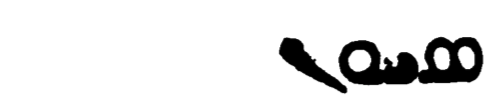
\includegraphics[height=10pt]{tables/099/08} } &
 Siwan &
 \textgreek{ἀρτεμίσιος[?]} &
 4
\\
 9 &
 \parbox[c]{5em}{
\includegraphics[height=10pt]{tables/099/09} } &
 Iijar &
 \textgreek{δαίσιος[?]} &
 5
\\
\midrule
 10 &
 \parbox[c]{5em}{
\includegraphics[height=10pt]{tables/099/10} } &
 Thamuz &
 \textgreek{πάνεμος[?]} &
 7
\\
 11 &
 \parbox[c]{5em}{
\includegraphics[height=10pt]{tables/099/11} } &
 Ab &
 \textgreek{λῶιος[?]} &
 1
\\
 12 &
% \parbox[c]{5em}{\includegraphics[height=\baselineskip]{tables/img/099_12} } &
% \includegraphics[height=\baselineskip]{tables/img/099_12} &
% \includegraphics[height=10pt]{tables/img/099_12} &
 \parbox[c]{5em}{
\includegraphics[height=10pt]{tables/099/12} } &
% \raisebox{-0.5\totalheight}{\includegraphics[height=10pt]{tables/img/099_12} } &
 Elul &
 \textgreek{γορπιαῖος[?]} &
 3
\\
 &
% \parbox[c]{5em}{\includegraphics[height=\baselineskip]{tables/img/099_13} } &
% \includegraphics[width=5em]{tables/img/099_13} &
% \includegraphics[height=10pt]{tables/img/099_13} &
 \parbox[c]{5em}{
\includegraphics[height=10pt]{tables/099/13} } &
 Elul alter. &
 \textgreek{γορπιαῖος δευτερος.[?]} &
 5
\\
\bottomrule
\end{tabular}
%
  \caption{Menses Chaldaei}
\end{table}
%\begin{table}[htbp]
%%%% Liber II p79
%%
%%% Count out columns for fixed-width source font
% 000000011111111112222222222333333333344444444445555555555666666666677777777778
% 345678901234567890123456789012345678901234567890123456789012345678901234567890
%
%% Select a general font size (uncomment one from the list)
%\tiny
%\scriptsize
%\footnotesize
%\small
%\normalsize
%% Center the whole table left-right
\centering
%% Modify separation between columns
%\setlength{\tabcolsep}{3pt}
%% Modify distance between rows
%\renewcommand{\arraystretch}{1.3}
%%
\begin{tabular}{@{}c c c@{} }
\toprule
\multicolumn{3}{c}{\Large\textsc{Tabella Characterismi Periodorum}}\\
\toprule
\multicolumn{1}{c}{Enneadeca-} &
\multicolumn{1}{c}{Character} &
\multicolumn{1}{c}{~}
\\
\multicolumn{1}{c}{eterides} &
\multicolumn{1}{c}{Enneadec.} &
\multicolumn{1}{c}{~}
\\
\midrule
 \rnum{i}    &  5 & 0   \\
 \rnum{ii}   &  1 & 19  \\
 \rnum{iii}  &  4 & 38  \\
 \rnum{iiii} &  7 & 57  \\
 \rnum{v}    &  3 & 76  \\
 \rnum{vi}   &  6 & 95  \\
 \rnum{vii}  &  2 & 114 \\
\bottomrule
\end{tabular}
%
\caption{Characterismi Periodorum}
%%%% Liber II p80
%%
%%% Count out columns for fixed-width source font
% 000000011111111112222222222333333333344444444445555555555666666666677777777778
% 345678901234567890123456789012345678901234567890123456789012345678901234567890
%
%\tiny
\scriptsize
%\footnotesize
%\small
%\normalsize
\centering
%% Modify separation between columns
\setlength{\tabcolsep}{1.6pt}
%% Modify distance between rows
\renewcommand{\arraystretch}{1.3}
%% Angle to rotate the headers
\newcommand{\ang}{75}
%%
\begin{tabular}{%
@{}r@{\hspace{0.3em}}r r  c
r@{~}l r@{~}l r@{~}l r@{~}l r@{~}l r@{~}l
r@{~}l
r@{~}l r@{~}l r@{~}l r@{~}l r@{~}l r@{~}l c
}
\toprule
\multicolumn{31}{c}{\Large\textsc{Tabula Neomeniarum Metonicarum}}\\
\multicolumn{31}{c}{\Large\textsc{in Mensibus Iulianis}}\\
\toprule
%~ &

\begin{rotate}{\ang}\hspace{0.3em}Anni Ennea-\end{rotate} &
\begin{rotate}{\ang}decaeteridis\end{rotate} &
\begin{rotate}{\ang}Cyclus Lunae\end{rotate} &
\begin{rotate}{\ang}Litera Dominica\end{rotate} &

\begin{rotate}{\ang}\textgreek{Εκατομβαιών}\end{rotate} & &
\begin{rotate}{\ang}\textgreek{Μεταγειτνιών}\end{rotate} & &
\begin{rotate}{\ang}\textgreek{Βοηδρομιών}\end{rotate} & &

\begin{rotate}{\ang}\textgreek{Πυανεψιών}\end{rotate} & &
\begin{rotate}{\ang}\textgreek{Μαιμακτηριών}\end{rotate} & &
\begin{rotate}{\ang}\textgreek{Ποσειδεών α}\end{rotate} & &
% $\overline\alpha$ does not work here (math mode does not render).
\begin{rotate}{\ang}\textgreek{Ποσειδεών β}\end{rotate} & &

\begin{rotate}{\ang}\textgreek{Γαμηλιών}\end{rotate} & &
\begin{rotate}{\ang}\textgreek{Ανθεστηριών}\end{rotate} & &
\begin{rotate}{\ang}\textgreek{Ελαφηβολιών}\end{rotate} & &

\begin{rotate}{\ang}\textgreek{Μουνυχιών}\end{rotate} & &
\begin{rotate}{\ang}\textgreek{Θαργηλιών}\end{rotate} & &
%\begin{rotate}{\ang}\textgreek{Σκιῤῥοφοριών}\end{rotate} & &
\multicolumn{3}{l}{\begin{turn}{\ang}\textgreek{Σκιῤῥοφοριών}\hspace*{1.2em}\end{turn}}

\\
\midrule
  &  1 &  7 & C &
 15&Iul & 14&Aug & 13&Sep & 12&Oct & 11&Nov & 10&Dec &
  \multicolumn{2}{c}{0} &
  9&Ian &  7&Feb &  9&Mar &  7&Apr &  7&Mai &  5&Iun
\\
† &  2 &  8 & B &
  5&Iul &  3&Aug &  2&Sep &  1&Oct & 31&Oct & 30&Nov &
 29&Dec &
 28&Ian & 26&Feb & 28&Mar & 26&Apr & 26&Mai & 24&Iun
\\
  &  3 &  9 & A &
 24&Iul & 22&Aug & 21&Sep & 20&Oct & 19&Nov & 18&Dec &
  \multicolumn{2}{c}{0} &
 17&Ian & 16&Feb & 16&Mar & 15&Apr & 14&Mai & 13&Iun
\\
  &  4 & 10 & G F &
 12&Iul & 11&Aug &  9&Sep &  9&Oct &  7&Nov &  7&Dec &
  \multicolumn{2}{c}{0} &
  5&Ian &  4&Feb &  5&Mar &  4&Apr &  3&Mai &  2&Iun
\\
† &  5 & 11 & E &
  2&Iul & 31&Iul & 30&Aug & 28&Sep & 28&Oct & 26&Nov &
 26&Dec &
 24&Ian & 23&Feb & 24&Mar & 23&Apr & 23&Mai & 21&Iun
\\
  &  6 & 12 & D &
 20&Iul & 19&Aug & 18&Sep & 17&Oct & 16&Nov & 15&Dec &
  \multicolumn{2}{c}{0} &
 14&Ian & 12&Feb & 14&Mar & 13&Apr & 12&Mai & 10&Iun
\\
  &  7 & 13 & C &
 10&Iul &  8&Aug &  7&Sep &  6&Oct &  5&Nov &  5&Dec &
  \multicolumn{2}{c}{0} &
  3&Ian &  2&Feb &  2&Mar &  8&Apr & 30&Apr & 30&Mai
\\
† &  8 & 14 & B A &
 28&Iul & 28&Iul & 26&Aug & 25&Sep & 25&Oct & 23&Nov &
 22&Dec &
 21&Ian & 20&Feb & 21&Mar & 20&Apr & 19&Mai & 18&Iun
\\
  &  9 & 15 & G &
 17&Iul & 16&Aug & 14&Sep & 14&Oct & 12&Nov & 12&Dec &
  \multicolumn{2}{c}{0} &
 10&Ian &  9&Feb & 10&Mar &  9&Apr &  8&Mai &  7&Iun
\\
† & 10 & 16 & F &
  7&Iul &  5&Aug &  4&Sep &  3&Oct &  2&Nov &  1&Dec &
 31&Dec &
 29&Ian & 28&Feb & 29&Mar & 28&Apr & 27&Mai & 26&Iun
\\
  & 11 & 17 & E &
 25&Iul & 24&Aug & 23&Sep & 22&Oct & 21&Nov & 20&Dec &
  \multicolumn{2}{c}{0} &
 19&Ian & 17&Feb & 18&Mar & 16&Apr & 16&Mai & 14&Iun
\\
  & 12 & 18 & D C &
 14&Iul & 12&Aug & 11&Sep & 10&Oct &  9&Nov &  8&Dec &
  \multicolumn{2}{c}{0} &
  7&Ian &  6&Feb &  7&Mar &  6&Apr &  5&Mai &  4&Iun
\\
† & 13 & 19 & B &
  3&Iul &  2&Aug & 31&Aug & 30&Sep & 29&Oct & 28&Nov &
 27&Dec &
 26&Ian & 24&Feb & 26&Mar & 25&Apr & 24&Mai & 23&Iun
\\
  & 14 &  1 & A &
 22&Iul & 21&Aug & 19&Sep & 19&Oct & 17&Nov & 17&Dec &
  \multicolumn{2}{c}{0} &
 15&Ian & 14&Feb & 15&Mar & 14&Apr & 13&Mai & 12&Iun
\\
  & 15 &  2 & G &
 12&Iul & 10&Aug &  9&Sep &  8&Sep &  7&Nov &  6&Dec &
  \multicolumn{2}{c}{0} &
  5&Ian &  3&Feb &  4&Mar &  2&Apr &  2&Mai & 31&Mai
\\
† & 16 &  3 & F E &
 30&Iul & 29&Iul & 28&Aug & 26&Sep & 26&Oct & 25&Nov &
 24&Dec &
 23&Ian & 21&Feb & 23&Mar & 21&Apr & 21&Mai & 19&Iun
\\
  & 17 &  4 & D &
 19&Iul & 17&Aug & 16&Sep & 16&Oct & 14&Nov & 13&Dec &
  \multicolumn{2}{c}{0} &
 12&Ian & 11&Feb & 12&Mar & 11&Apr & 10&Mai &  8&Ian
\\
† & 18 &  5 & C &
  8&Iul &  7&Aug &  5&Sep &  5&Oct &  3&Nov &  3&Dec &
  1&Ian &
 31&Ian &  1&Mar & 31&Mar & 30&Apr & 29&Mai & 28&Iun
\\
  & 19 &  6 & B &
 27&Iul & 26&Aug & 24&Sep & 24&Oct & 22&Nov & 22&Dec &
  \multicolumn{2}{c}{0} &
 20&Ian & 19&Feb & 20&Mar & 19&Apr & 18&Mai & 17&Iun
\\
\bottomrule
\addlinespace
& & \multicolumn{29}{l}{\footnotesize \super{†} \textgreek{ἐμβ. [?]}}\\
\end{tabular}
\caption{Neomeniarum Metonicarum in Mensibus Iulianis}

%%%% Liber II p82
%%
%%% Count out columns for fixed-width source font
% 000000011111111112222222222333333333344444444445555555555666666666677777777778
% 345678901234567890123456789012345678901234567890123456789012345678901234567890
%
%% Select a general font size (uncomment one from the list)
%\tiny
%\scriptsize
%\footnotesize
%\small
\normalsize
%% Center the whole table left-right
\centering
%% Modify separation between columns
%\setlength{\tabcolsep}{1.6pt}
%% Modify distance between rows
%\renewcommand{\arraystretch}{1.3}
%%
\begin{tabular}{@{}c c c c c@{} }
\toprule
\multicolumn{5}{c}{\Large\textsc{Linea \textgreek{μεταπτώσεως} Metonicae}}\\
\midrule
\multicolumn{1}{c}{Anni collecti} &
\multicolumn{1}{c}{Dies} &
\multicolumn{1}{c}{Scru. diur.} & % [Abbriv]
\multicolumn{1}{c}{Momenta}
\\
\midrule
  19 &  0 & 18 & 57 \\
  38 &  0 & 37 & 38 \\
  57 &  0 & 56 & 19 \\
  76 &  1 & 15 &  0 \\
  95 &  1 & 33 & 57 \\
 114 &  1 & 52 & 38 \\
 133 &  2 & 11 & 19 \\
 152 &  2 & 30 &  0 \\
 171 &  2 & 40 & 57 \\
 190 &  3 &  7 & 38 \\
 209 &  3 & 26 & 19 \\
 228 &  2 & 45 &  0 \\
 247 &  4 &  3 & 57 \\
 266 &  4 & 22 & 38 \\
 285 &  4 & 41 & 19 \\
 304 &  5 &  0 &  0 \\
\midrule
 608 & 10 &  0 &  0 \\
1216 & 20 &  0 &  0 \\
1824 & 30 &  0 &  0 \\
2432 & 40 &  0 &  0 \\
2736 & 45 &  0 &  0 \\
\bottomrule
\end{tabular}
%
\caption{Linea metaptoseos Metonicae}

%%
%%
%\end{table}

%\begin{table}[htbp]
%%%% Liber II p67, PDF 150
%%
%% Conversion of Νεομηνιαι της Οκταετηριδος καθ´ εκαστον ετος
%% eliminating most of the Greek.
%% - The column headers (ἔτος προτον, etc) are simply year numbers
%% - The body of the table consists of Greek numbers for days, and the names
%%   of the months, which are also listed in the first columns.
%%   The numbers are converted to arabic numerals, and the names of the months
%%   are indexed with roman numerals, and a column of those roman numerals is
%%   added to the left of the column with the Greek names of the months.
%%
%%% Count out columns for fixed-width source font
% 000000011111111112222222222333333333344444444445555555555666666666677777777778
% 345678901234567890123456789012345678901234567890123456789012345678901234567890
%
%% Select a general font size (uncomment one from the list)
%\tiny
%\scriptsize
%\footnotesize
%\small
%\normalsize
%% Center the whole table left-right
\centering
%% Modify distance between rows
\renewcommand{\arraystretch}{1.2}
%% Modify separation between columns
\setlength{\tabcolsep}{2.0pt}
%
\begin{tabular}{@{}cl llllllll@{}}
\toprule
\multicolumn{2}{ c }{~} &
\multicolumn{8}{ c }{annum}
\\
\cmidrule{3-10}
\multicolumn{2}{ c }{Mensis lunaris} &
\multicolumn{1}{c}{1} &
\multicolumn{1}{c}{2} &
\multicolumn{1}{c}{3} &
\multicolumn{1}{c}{4} &
\multicolumn{1}{c}{5} &
\multicolumn{1}{c}{6} &
\multicolumn{1}{c}{7} &
\multicolumn{1}{c}{8}
\\
\midrule
\textsc{vii} & \textgreek{γαμηλιών} &
 1.\textsc{vii} &
25.\textsc{vi} &
18.\textsc{vi} &
 8.\textsc{vii} &
 1.\textsc{vii} &
26.\textsc{vi} &
16.\textsc{vii} &
 8.\textsc{vii}
\\
\textsc{viii} & \textgreek{ανθεστηριών} &
 1.\textsc{viii} &
23.\textsc{vii} &
15.\textsc{vii} &
 8.\textsc{viii} &
 1.\textsc{viii} &
23.\textsc{vii} &
15.\textsc{viii} &
 8.\textsc{viii}
\\
\textsc{ix} & \textgreek{ἐλαφηβολιών} &
 1.\textsc{ix} &
23.\textsc{viii} &
15.\textsc{viii} &
 7.\textsc{ix} &
30.\textsc{viii} &
23.\textsc{viii} &
15.\textsc{ix} &
 7.\textsc{ix}
\\
\midrule
\textsc{x} & \textgreek{μυονυχιών} &
30.\textsc{ix} &
22.\textsc{ix} &
14.\textsc{ix} &
 7.\textsc{x} &
30.\textsc{ix} &
22.\textsc{ix} &
14.\textsc{x} &
 7.\textsc{x}
\\
\textsc{xi} & \textgreek{θαργηλιών} &
30.\textsc{x} &
22.\textsc{x} &
14.\textsc{x} &
 6.\textsc{xi} &
29.\textsc{x} &
22.\textsc{x} &
14.\textsc{xi} &
 6.\textsc{xi}
\\
\textsc{xii} & \textgreek{σκιῤῥοφοριών} &
29.\textsc{xi} &
21.\textsc{xi} &
14.\textsc{xi} &
 6.\textsc{xii} &
24.\textsc{xi} &
21.\textsc{xi} &
13.\textsc{xii} &
 6.\textsc{xii}
\\
\midrule
\textsc{i} & \textgreek{ἑκατομβαιών} &
29.\textsc{xii} &
21.\textsc{xii} &
13.\textsc{xii} &
 6.\textsc{i} &
29.\textsc{xii} &
21.\textsc{xii} &
13.\textsc{i} &
 5.\textsc{i}
\\
\textsc{ii} & \textgreek{μεταγειτνιών} &
28.\textsc{i} &
20.\textsc{i} &
13.\textsc{i} &
 5.\textsc{ii} &
28.\textsc{i} &
20.\textsc{i} &
12.\textsc{ii} &
 5.\textsc{ii}
\\
\textsc{iii} & \textgreek{βοηδρομιών} &
28.\textsc{ii} &
20.\textsc{ii} &
12.\textsc{ii} &
 5.\textsc{iii} &
28.\textsc{ii} &
20.\textsc{ii} &
12.\textsc{iii} &
 4.\textsc{iii}
\\
\midrule
\textsc{iv} & \textgreek{πυανεψιών} &
27.\textsc{iii} &
19.\textsc{iii} &
12.\textsc{iii} &
 5.\textsc{iv} &
27.\textsc{iii} &
20.\textsc{iii} &
11.\textsc{iv} &
 4.\textsc{iv}
\\
\textsc{v} & \textgreek{μαιμακτηριών} &
27.\textsc{iv} &
19.\textsc{iv} &
11.\textsc{iv} &
 4.\textsc{v} &
27.\textsc{iv} &
19.\textsc{iv} &
11.\textsc{v} &
 3.\textsc{v}
\\
\textsc{vi} & \textgreek{ποσειδεών} $\overline{\alpha}$&
26.\textsc{v} &
18.\textsc{v} &
11.\textsc{v} &
 3.\textsc{vi} &
26.\textsc{v} &
19.\textsc{v} &
11.\textsc{vi} &
 3.\textsc{vi}
\\
\textsc{vi} & \textgreek{ποσειδεών} $\overline{\beta}$&
26.\textsc{vi} $\overline{\alpha}$ &
    \multicolumn{1}{c}{$\circ$} &
10.\textsc{vi} &
    \multicolumn{1}{c}{$\circ$} &
    \multicolumn{1}{c}{$\circ$} &
18.\textsc{vi} &
    \multicolumn{1}{c}{$\circ$} &
\multicolumn{1}{c}{~}\\
\bottomrule
\end{tabular}
%
\caption{Neomeniae octaeteridai Harpali per annum}

%\end{table}

Donec maximus, leo nec accumsan laoreet, nulla nibh posuere neque, at malesuada
mauris leo vitae magna. Mauris vel nisl vitae est congue finibus.
Praesent suscipit suscipit erat sit amet aliquam. Maecenas nunc metus, varius at
sodales eget, pellentesque in risus.
Donec vel nisi eget arcu condimentum blandit non non urna.
Phasellus quis fermentum lacus.
Cras orci nulla, venenatis vitae sapien eu, cursus pulvinar erat.
Suspendisse facilisis orci eget ante cursus rhoncus vel quis neque.
Integer eu commodo tellus.
Nullam sed tortor id lacus imperdiet accumsan.
Sed malesuada nisi vel justo pretium bibendum.
Nulla ultrices, turpis sed finibus finibus, tortor libero fermentum dolor,
in mollis ante magna ut neque.
\end{document}
